\chapter{Asking Atlanta Millionaires How They Got Rich}

This lecture is not mathematical in the narrow blackboard sense, but it does unfold a real analytic structure. We move from visible wealth to the mechanisms said to produce it, from isolated success stories to recurring commercial patterns, and finally from business method to the deeper question of personal foundation. The notes below preserve that order. We begin with spectacle, pass through scaling, marketing, capital, and advice, and end with the sharper claim that financial freedom is built not only on tactics but on fit, discipline, and the capacity to bear the second-order consequences of success.

\section{Atlanta Wealth as a Field Site}

The video opens with a teaser: an extraordinary house, a promise to walk up to its owner, and the practical question that governs the whole lecture, namely what sort of work could support that level of visible affluence. This is important structurally. The lecture does not begin with doctrine. It begins with a field test. We are asked to treat houses, cars, and neighborhoods as clues, then to press through the surface until the mechanism is named.

The first concrete point is not yet an answer but a method. The host goes to the door, explains the channel, requests permission, and then starts gathering parameters: how long has the owner been in Atlanta, what does he do, how many businesses does he own, and what has the best year looked like. The lecture is already quantitative. It wants us to keep count.

\section{Serial Entrepreneurship and the First Scale Marker}

The first homeowner reports roughly fourteen years in Atlanta, presents himself in substance as a serial entrepreneur, and says that he currently owns six businesses. The first major numerical anchor is then produced: the best single year he names is \$15 million. Immediately after that, the lecture asks the more general question: how does someone become a millionaire in 2024? Instead of answering directly, the narration widens the lens and re-situates the inquiry at the level of the city.

\begin{align}
N_{\text{ATL,millionaires}} &\approx 20{,}000,\\
B_{\text{serial}} &= 6,\\
Y^{\max}_{\text{serial}} &= \$15\,\mathrm{M}.
\end{align}

The function of these numbers is not merely decorative. They turn the opening spectacle into a searchable terrain. Atlanta is presented as a dense environment of wealthy operators, and the chapter therefore proceeds not as a single profile but as a sequence of cases from which common rules may be extracted. The lecture is telling us, in effect, that if there are enough such cases in one city, we may treat the city as a laboratory of commercial behavior.

\section{Producer, Consumer, and the Geometry of Attention}

The Lamborghini interview supplies the lecture's first real theory. The entrepreneur reports more than a decade and a half as a full-time entrepreneur, around eight years in marketing, and recent annual results a little above \$10 million. He also presents a severe background of hardship and explicitly rejects the idea that he came from money. This matters because the lecture now wants a sharper contrast than mere biography. It wants a distinction of orientation.

When asked whether he is a buyer or a seller, he answers that he is both, but immediately qualifies the point: he buys information in order to become better, yet prefers to stand on the side of production rather than consumption. This is the moment at which the lecture changes register. It is no longer only asking who made money. It is asking from which side of the market one tries to live.

We may formalize that contrast in a minimal way. Let \(C\) denote a consumer orientation, \(P\) a producer orientation, and let \(A\) denote the level of public awareness attached to one's work. The lecture's claim is not that consumption disappears, but that consumption should become instrumental to later production.

\begin{equation}
P > C \qquad \text{in strategic importance for wealth formation.}
\end{equation}

The entrepreneur then adds the image of horse blinders. The point is not aesthetic. It is a model of attention. If one keeps looking sideways at the cultural trivia of other people's victories, one loses the lane of one's own race. In a lecture of this kind, the metaphor does real analytic work: attention is treated as a scarce resource that must be shielded from lateral distraction.

\begin{figure}[h]
\centering
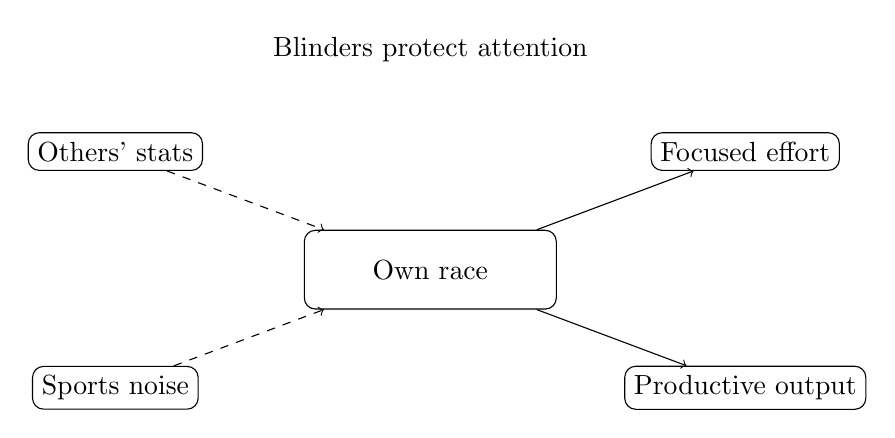
\begin{tikzpicture}
\node[draw, rounded corners] (left) at (-4,1.5) {Others' stats};
\node[draw, rounded corners] (leftb) at (-4,-1.5) {Sports noise};
\node[draw, rounded corners, minimum width=3.2cm, minimum height=1cm] (center) at (0,0) {Own race};
\node[draw, rounded corners] (right) at (4,1.5) {Focused effort};
\node[draw, rounded corners] (rightb) at (4,-1.5) {Productive output};

\draw[->] (center) -- (right);
\draw[->] (center) -- (rightb);
\draw[dashed, ->] (left) -- (center);
\draw[dashed, ->] (leftb) -- (center);

\node at (0,2.8) {Blinders protect attention};
\end{tikzpicture}
\caption{A transcript-based reconstruction of the blinder metaphor. The lecture treats wealth-building as an attentional problem as well as a financial one.}
\end{figure}

\subsection{Question \& Answer: Why Do Most Businesses Fail to Scale?}

The lecture then poses a sharper problem. If more than \(90\%\) of businesses fail to survive five years, what is the most common mistake? The answer given is lack of marketing. That answer is easy to trivialize if we move too quickly. The lecture does not mean ``advertise a little more.'' It means that excellent execution without visibility is commercially indistinguishable from non-existence.

\begin{equation}
p_{\text{fail by 5 yr}} > 0.9
\end{equation}

\begin{equation}
Q_{\text{offer}} + A_{\text{low}} \Rightarrow F_{\text{high}},
\end{equation}
where \(Q_{\text{offer}}\) denotes the quality of the underlying offer, \(A\) denotes awareness, and \(F\) denotes failure risk.

We can write the lecture's reasoning as a short derivation.

\begin{enumerate}
\item A business may be extremely good at what it does.
\item If awareness \(A\) is low, the market does not know the business exists.
\item If the market does not know the business exists, growth stalls.
\item Stalled growth, repeated over time, raises failure risk \(F\).
\item Therefore marketing is part of the firm's survival structure, not an optional cosmetic layer.
\end{enumerate}

A simple heuristic update rule captures the same point:

\begin{equation}
A_{t+1} = A_t + m_t,
\end{equation}
where \(m_t\) is sustained marketing effort or marketing spend at stage \(t\). The lecture's claim is that when \(m_t\) is neglected for too long, awareness does not compound, and the probability of scale fails to compound with it.

\begin{equation}
A_{\uparrow} \Rightarrow \Pr(\text{scale})_{\uparrow}.
\end{equation}

This is the first fully worked mechanism in the lecture. Good work alone is not sufficient; good work must enter the field of public recognition.

\section{Advice, Social Proof, and the Problem of Small Minds}

The same interview now turns from market visibility to the social handling of ambition. The entrepreneur says that the fastest way to kill a big dream is to tell it to a small mind. The lecture is not merely praising confidence. It is refining the problem of reference classes. Whose judgments are relevant to our next move?

Here the mechanism is social rather than financial. Family may love us, but loving us is not the same as having built the kind of enterprise we want to build. A coworker may be sincere, but sincerity is not competence in entrepreneurship. The lecture therefore imposes a filter on advice: if one wants to become a millionaire, one should learn from those who have already operated at that level rather than from those whose incentives are tied to caution or stasis.

This is also the point at which the host recaps. The recap matters because it tells us what the lecture itself regards as portable. The interview is not left as one man's biography. It is condensed into a theorem-like phrase: big ambition must be protected from the interpretive habits of small minds.

\section{Capital, Timing, and the Real-Estate Developer's View of Scale}

The real-estate developer widens the frame. The first question is practical: can one get started in real estate without much money? The answer is blunt. Real estate is expensive, and one does need capital. That is the first hard correction. The lecture does not offer a false low-barrier dream in a capital-intensive field.

The same speaker then reports a long career in commercial real-estate development and names a best year of \$100 million. He is next asked how one scales from eight to nine figures. His answer is concise and unexpectedly deflationary: timing matters. Already the lecture has moved beyond hustle rhetoric. It is making room for circumstance, cycle, and luck.

\begin{align}
T_{\text{RE}} &= 25\,\text{years},\\
Y^{\max}_{\text{RE}} &= \$100\,\mathrm{M}.
\end{align}

When the conversation turns to billionaires, he presses the deflation farther. Wealth, he says, does not automatically certify intelligence; many people get lucky. That in turn sets up one of the lecture's cleanest definitions.

\begin{definition}
Beliefs are what one thinks is true. Values are what one thinks is important.
\end{definition}

\begin{equation}
Bel = \text{what one thinks is true},\qquad Val = \text{what one thinks is important}.
\end{equation}

The claim is subtle. Commercial judgment is not only about having more facts. It is also about ranking what matters. That prepares the way for the lecture's discussion of capital raising. The developer argues that there is more money in the world looking for good business plans than there are genuinely good business plans.

\begin{equation}
K_{\text{available capital}} > G_{\text{good business plans}}.
\end{equation}

This is not a numerical theorem. It is a market-structure claim. The bottleneck is not money in the abstract; it is the scarcity of plans that survive rapid scrutiny. The lecture gives the screening criteria in ordinary language, and we may write them schematically as follows:

\begin{enumerate}
\item The plan must make sense at the level of margins.
\item It must make sense at the level of cost structure.
\item It must have a legitimate pathway to growth.
\item It must show why the investor's money will come back with a sensible return.
\end{enumerate}

If we write \(R\) for the return legible to the investor, the lecture's commercial logic is

\begin{equation}
G_{\text{plan}} \Rightarrow \text{coherent margins} \Rightarrow \text{coherent growth path} \Rightarrow R_{\text{credible}}.
\end{equation}

The same interview then pivots once more, from wealth to happiness. The speaker jokes about the age at which he became a millionaire, then says that he has not tracked that boundary because it is not what mattered most to him. What mattered was becoming happy, discovering that he enjoyed development, and finding a domain in which a prior skill --- resource management learned in the restaurant world --- could be carried into a new vocation. This is crucial for the chapter's later ending: a wealthy life is being described not only in terms of money but in terms of fit.

\section{Question \& Answer: What Should Someone at Rock Bottom Actually Do?}

The final entrepreneur returns the lecture to urgency. He says he made his first million at twenty-nine, but also says that he was once homeless and broke, and that he spent the years from roughly twenty-four to twenty-six getting back on his feet. This gives the lecture a very different kind of authority. It is no longer merely describing how wealthy people allocate capital. It is now trying to diagnose what should happen first when there is no money at all.

\begin{equation}
a_{\text{first million}} = 29.
\end{equation}

The question is explicit: what actionable step should a person at rock bottom take if he wants to become financially free? The answer is also explicit: the first issue is not money. The first issue is the self.

\begin{equation}
H_{\text{bad}} \Rightarrow D_{\text{bad}} \Rightarrow \text{financial instability},
\end{equation}
where \(H_{\text{bad}}\) denotes destructive habits and \(D_{\text{bad}}\) the bad daily decisions that flow from them.

The speaker's logic unfolds in stages.

\begin{enumerate}
\item What looks like a money problem is often a personal problem.
\item Personal disorder appears as trauma, bad habits, and repeated bad decisions.
\item Those repeated decisions place the individual in a financially unstable state.
\item The first move is subtractive: identify what must be cut out.
\item Only after that do we move to acquisition, especially to a skill that directly earns, namely selling.
\item Business building should then occur on top of a repaired foundation rather than on top of unresolved chaos.
\end{enumerate}

We may compress that chain into a single lecture-equation:

\begin{equation}
\text{self-repair} \Rightarrow S_{\text{sell}} \Rightarrow \text{foundation} \Rightarrow \text{financial progress}.
\end{equation}

This is the strongest prescriptive moment in the lecture. It is not optimistic in a cheap way. It is sequential. It says that the order matters. One does not first decorate oneself with ambition and only later clean up the underlying life. One cleans, stabilizes, learns a high-leverage skill, and only then builds.

\section{Mindset, Skill Set, and the Price of Success}

The lecture now sharpens its ranking: what matters more, mindset or skill set? The answer is mindset. The reason is selection. A poor mindset chooses the wrong arena, chases someone else's strategy, misreads the self, and therefore acquires the wrong skills for the wrong reasons.

\begin{equation}
M \succ S,
\end{equation}
and more precisely,
\begin{equation}
M \Rightarrow \text{choose}(S_{\text{fit}}).
\end{equation}

This is not a denial of skill. It is a claim about ordering. Skill without self-knowledge gets assigned badly. The lecture's examples are blunt: an introvert may copy a sales career he does not suit; someone may chase influence without the temperament, consistency, or presence required for it. In that sense, mindset is not mere positivity. It is correct self-reading.

The same speaker then gives a sharp piece of financial advice: spend money, but spend it as a tool. Spend it to gain information, to widen the network, and to enter environments that would otherwise be inaccessible. The underlying principle is that money should be deployed into feedback and access, not merely displayed.

The closing theme, however, is not upward mobility but the burden of arrival. When asked about a deep life quote, the entrepreneur answers with ``more money, more problems'' and then explains why. The lecture refuses to leave wealth as a one-directional gain. It adds a second layer. Money creates options, but it also changes expectations, relationships, judgments, and the emotional texture of ordinary life.

\begin{equation}
\text{wealth}_{1\text{st order}} \Rightarrow \text{optionalities},\qquad
\text{wealth}_{2\text{nd order}} \Rightarrow \text{new burdens}.
\end{equation}

In that final turn the lecture becomes genuinely book-like. It ceases to be only a survey of rich people and becomes a meditation on the instability of aspiration itself. Success does not freeze the world around us. It changes the world around us, and it changes us with it.

\section{Summary}

The lecture proceeds by live encounter, but it yields a stable structure. Wealth first appears as a visible mystery, then as a set of measurable outcomes, then as a pattern of production, focus, marketing, advice selection, capital credibility, and personal fit. The strongest recurring claims are these: scale requires visibility; ambition must be protected from the wrong audience; capital chases credible plans more eagerly than vague ideas; and financial repair begins with the self before it flowers into strategy.

The last movement matters most. We are not finally told that money solves everything. We are told that money is built on habit, judgment, and alignment, and that even when it arrives it brings a second-order world of obligations and frictions with it. That is why the lecture holds together. It does not merely praise wealth. It studies its mechanism and its cost.